\documentclass[a4wide]{report}

\usepackage{amsmath}
\usepackage[a4paper, total={7in, 10.2in}]{geometry}
\usepackage{graphicx}
\usepackage[portuguese]{babel}
\usepackage[utf8]{inputenc}


\begin{document}

\noindent
{\bf Lincoln Martins de Oliveira (ES 90693) - Mini-relatório 01 (\today)}

\begin{quote}

\centering

\bf Mecanismos de transfer\^encia de calor

\end{quote}

%\section{Introdução}
%\label{intro}

\vspace{0.5cm}

	Quando você coloca uma colher em uma caneca contendo leite quente, a colher se aquece e o leite 
se esfria e ambos os corpos lentamente encaminham-se para atingir o equilíbrio térmico. O contato 
que ocasiona essas variações de temperatura é basicamente uma movimentação de energia entre um 
corpo e outro. A transferência de energia gerada apenas por diferença de temperatura e chamada de 
transferência de calor ou fluxo de calor, e a energia transferida desta forma e designada por calor.
	
	Os três processos de propagação de calor são a condução, a convecção e a radiação.
A condução ocorre no interior de um corpo ou entre dois ou mais corpos em contato. A convecção 
depende do movimento de massas de uma região para outra. A radiação é a propagação de calor que 
ocorre por meio da radiação eletromagnética, sem que seja necessária a presença de mátria entre 
os corpos. Seja por qualquer um desses processos de transferência, o calor sempre fluirá de um 
corpo que possui maior temperatura para o corpo com menor temperatura.



\begin{quote}

\centering

\bf Condução térmica

\end{quote}

	Suponha que uma pessoa esteja segurando a extremidade A de uma barra metálica e a outra 
extremidade, B, esteja em contato com uma chama. Com o passar do tempo essa pessoa nota que a
temperatura na extremidade A se elevou, isso e deve a maior agitação das moléculas ou átomos da 
extremidade B, aquecida pela chama. Parte dessa energia adquirida da chama por B e transferida 
para as partículas da região vizinha por meio do choque entre as partículas que constituem o 
corpo, ao receber essa energia as partículas passam a vibrar com maior ímpeto, esta propaga 
energia para a subsequente e assim, sucessivamente como mostrada na figura ~\ref{barra_moleculas}.



\begin{figure}[h]
\centering
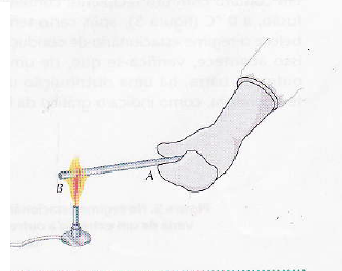
\includegraphics[width=0.23\textwidth]{barra_aquecida}
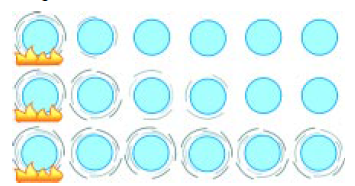
\includegraphics[width=0.23\textwidth]{moleculas}
\caption{Barra sendo aquecida e ampliação das moleculas que a compoem mostrando seu comportamento microscópio.
Figuras extraídas da Referência~\cite{Cur}.}
\label{barra_moleculas}
\end{figure}
	Conforme seja a constituição atômica de uma substancia, a agitação térmica pode ser 
transmitida de um átomo parra outro com maior o menor facilidade, metais, por exemplo, são bons 
condutores de calor, no entanto outras substâncias, como o isopor, o vidro, a borracha, o ar a 
madeira, a lã, entre outros são maus condutores de calor, ou seja, isolantes térmicos.
\begin{quote}

\centering

\bf Fluxo de calor

\end{quote}

\begin{figure}[h]
\centering
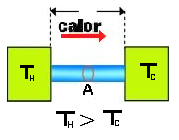
\includegraphics[width=0.23\textwidth]{fluxo}
\caption{A figura mostra um sistema formado por dois corpos a temperaturas diferentes ligados por uma barra.
Figuras extraídas da Referência~\cite{Cur}.}
\label{fluxxo}
\end{figure}

Imaginemos uma barra metálica de comprimento L e cuja área de seção reta transversal seja A, e as
quais sejam mantidas em temperaturas diferentes, como na figura ~\ref{fluxxo}.

Nessas condições o calor fluirá do corpo mais quente (Th) para o corpo mais frio (Tc) através da
barra. A quantidade de calor (Q) que transpassa a seção reta da barra em um intervalo e 
tempo ($\Delta$  t ) é chamada de fluxo de calor.

Representamos a taxa de transferência de calor H por meio da equação abaixo, no SI sua 
unidade de medida é dada por joule por segundo ($\frac{J}{s}$) ou watt (W):
\begin{equation}
\centering
H   =   \frac{Q}{\Delta t}
~~~~~~~.
\label{equacao_fluxo}
\end{equation}

\begin{quote}

\centering

\bf Lei da condução térmica ou lei de Fourier

\end{quote}

Consideremos agora o mesmo esquema apresentado anteriormente representado pela figura ~\ref{fluxxo}, 
vimos que o fluxo de calor H depende da área de seção reta transversal A da barra, do 
comprimento L da mesma, da diferença de temperatura $\Delta T$ $=$ $(Th$ $-$ $Tc)$ e da natureza o material que
compõe a barra.

Por meio de um experimento verifica-se que, para um determinado material, a taxa de transferência 
de calor e tanto maior quanto mais extenso for à área de seção reta transversal da barra (A), 
quão grande for à diferença de temperatura $\Delta$T e quanto menor o comprimento L da barra.

Deste modo podemos enunciar a lei de Fourier da seguinte maneira:
\begin{quote}

\centering

"Em regime estacionário, a corrente de calor por condução em um material uniforme é diretamente 
proporcional a A e a $\Delta$T, e inversamente proporcional ao comprimento L"

\end{quote}

Essa lei Relaciona o fluxo de calor com as variáveis que o determinam. Essa relação e dada por:

\begin{equation}
\centering
H   =   \frac{Q}{\Delta t} = KA \frac{\Delta T}{L}
~~~~~~~.
\label{equacao_fourier}
\end{equation}

\begin{table}[!h]
\centering
 \begin{tabular}{ccc}
  \hline\\[-0.37cm]
  \hline
  Material                 & Massa específica ()          & Condutividade térmica (W/mK)  \\ \hline
  Aumínio              &	2800                                         &  204                    \\
  Cobro                  &	9000                                         & 372                     \\
 Ligas                &        12250                                       & 35                  \\
 Aço, ferro          &	         7800                                & 52              \\
 Zinco                 &	 7200                                        &  110   \\
 Basalto, granito     &	          3000                                         &  3.5 \\
 Calcário, mármore      &        2700                                      &   2.5   \\
  arenito               &	2060                                         &  1.6 \\
 Ar                     & 	1.2                                          & 0.023 \\
 \hline\\[-0.37cm]
  \hline
\end{tabular}
\caption{Alguns dos coeficientes de condutibilidade térmica de alguns materiais presentes no nosso dia a dia.
Observe que esses valores valem somente no seco.Tabela extraídas da Referência~\cite{protolab}.}
\label{Ks}
\end{table}

A constante de proporcionalidade K é conhecida como coeficiente de condutibilidade térmica e 
define o material por onde o calor flui por condução. Se o material apresentar valor de K elevado,
significa que ele é bom condutor de calor, já se o material apresentar valor de K baixo remete que 
o material e mau condutor de calor ou isolante térmico. Algums de seus valores estao representados 
na tabela ~\ref{Ks}.

\begin{thebibliography}{99}

\bibitem{ramalho} Ramalho. Nicolau. Toledo. Os Fundamentos da Física 2, termologia ótica e ondas.

\bibitem{Cur} Curso de formação de operadores de refinaria física aplicada termometria, calorimetria e transmissão de calor. 

\bibitem{antonio} MÁXIMO, Antônio; ALVARENGA, Beatriz. Curso de Física. São Paulo: Scipione, 2006. V1.

\bibitem{sears} SEARS, ZEMANSKY, Física, Vol 2, 10ª Edição, Pearson, 2003.

\bibitem{educador} http://educador.brasilescola.uol.com.br/estrategias-ensino/experimento-sobre-correntes-conveccao.htm (23/03/2018)

\bibitem{protolab} http://www.protolab.com.br/Tabela-Condutividade-Material-Construcao.htm (23/03/2018)

\end{thebibliography}

\end{document}